% Important: The shell-escape flag is required for the Minted package.
% Please compile this document with 'pdflatex -shell-escape main.tex'.
% If you are using another IDE, you may be able to specify this in the
% options or to provide an option like '% !TEX option = -shell-escape'
% in this file, depending on your builder. See the README.md for more.

% Don't put any content in here.
% Don't even include content files by using \input or \inlcude.
% Put your content into components/text.tex or include it there using \input.
% You probably want to modify the following files:
%   components/info.tex             contains the author, title etc.
%   components/settings.tex         contains the packages and settings.
%   components/commands.tex         contains helpful custom commands.
%   components/glossary.tex         contains an explanation of the used terms.
%   components/acknowledgements.tex contains the acknowledgements.
%   components/quote.tex            contains a quote.
%   components/abstract.tex         contains the abstract of the document.
%   components/text.tex             includes the actual content of the document.
%   chapters/                       contains the main text.
%   bibliography/literature.bib     contains the BibTeX entries.
%   images/                         contains all your content-related images.
%
% You probably don't need to change anything in the following files:
%   components/cover.tex            formats the front cover of the document.
%   components/titlepage.tex        formats the title page of the document.
%   components/disclaimer.tex       formats the disclaimer page.
%   styles/                         contains style elements (e.g. logos).
%   main.tex                        contains the top-level code structure.
%   README.md                       contains information about this template.

\documentclass[11pt,
              a4paper,
              index=totoc,
              headsepline,
              footsepline,
              BCOR=12mm,
              DIV=13,
              bibliography=totoc]{scrbook}

% KOMA scrbook options:
%  index=totoc: include an entry for the index in the table of contents.
%  headsepline: use horizontal line under heading.
%  footsepline: use horizontal line above footer.
%  BCOR: binding correction (e.g.: BCOR=12mm)
%  DIV: Number of sheet sections (used for layout) (e.g.: DIV=13)

% !TEX root = ../main.tex
% Set here the title, authors and other stuff to be used for the cover
% This file is used by MAIN.TEX

% set title, authors and stuff for the cover
\def\university{Universidad de Los Andes}
\def\universityLogo{styles/uniandes-logo}
\def\program{Master of Information Engineering}
%% \def\programLogo{styles/uniandes-logo}
\def\doctype{Master's Thesis}

\def\title{Network Aware Elastic Key-Splitting in Distributed Stream Processing Systems}
\def\author{Diva Mercedes Martínez Laverde}
\def\examinerOne{ToFind}
\def\examinerTwo{ToFind}
\def\assistantAdvisor{Nicolás Cardozo Álvarez Ph.D.}
\def\date{June 2019}

\def\keywords{{stream-processing}}

% The following are used for the PDF metadata, by default the same as above.
\def\metaTitle{\title}
\def\metaAuthor{\author}
\def\metaSubject{\doctype\ -\ \university}
\def\metaKeywords{\keywords}

% text to appear in the footer
\def\footertext{}

% !TEX root = ../main.tex
% Included by MAIN.TEX

%--------------------------------------------------
% Fonts and page setup
%--------------------------------------------------

% Default font
\usepackage{palatino}

% Enable special PostScript fonts (optional)
% \usepackage{pifont}

% Manipulate the footer
\usepackage{scrlayer-scrpage}
\usepackage{scrhack}
\pagestyle{scrheadings}
\ifoot[\footertext]{\footertext} % \footertext set in INFO.TEX

% Set the font for the section headings
\renewcommand{\sectfont}{\normalfont \bfseries}

% Conditional commands in LaTeX documents, used for the \clearemptydoublepage.
\usepackage{ifthen}

% Typeset text in multiple columns (optional)
% \usepackage{multicol}

% Rotation tools, including rotated full-page floats (optional)
\usepackage{rotating}


%--------------------------------------------------
% Document structure
%--------------------------------------------------

% Standard LaTeX package for creating indexes
\usepackage{makeidx}

% Pro­duce hy­per­text links in the doc­u­ment (recommended)
\usepackage{hyperref}

%--------------------------------------------------
% Bibliography
%--------------------------------------------------

% Set the bibliography style (default: plain)
\bibliographystyle{plain}

% Special biblography package (nice to have)
% \usepackage{natbib}


%--------------------------------------------------
% Graphics and floats
%--------------------------------------------------

% Enhanced support for graphics (recommended)
\usepackage{graphicx}
% Path to the figures directory (default: {figures/})
% Multiple entries are allowed, e.g. {{figures1/}{figures2/}}.
\graphicspath{{figures/}}

% Improved interface for floating objects (optional)
\usepackage{float}

% To use the subfigures (optional)
\usepackage{subcaption}


%--------------------------------------------------
% Mathematics
%--------------------------------------------------

% AMS mathematical facilities for LaTeX (recommended)
\usepackage{amsmath}

% TeX fonts from the American Mathematical Society (recommended)
\usepackage{amsfonts}

% Some extra math symbols (optional)
% \usepackage{amssymb}

% Extended maths fonts for LaTeX (optional)
% \usepackage{yhmath}

% Provide math delimiters whose size can be computed automatically (optional)
% \usepackage{commath}


%--------------------------------------------------
% Source code and algorithms
%--------------------------------------------------

% Source code typesetting
% \usepackage{listings} % (optional - alternative)
\usepackage[newfloat]{minted} % (recommended)
% Set global Minted options
\setminted{linenos, autogobble, frame=lines, framesep=2mm}
% Inline C++ (optional)
\newcommand{\incpp}[1]{\mintinline{c++}{#1}}
\newenvironment{code}{\captionsetup{type=listing}}{}
\SetupFloatingEnvironment{listing}{name=Source Code}

% Typeset algorithms - pseudocode (optional)
% \usepackage{algorithmicx}
% \usepackage{algpseudocode}
% Normal arrow comments
% \algrenewcommand{\algorithmiccomment}[1]{\hfill$\rightarrow$ #1}


%--------------------------------------------------
% Tables
%--------------------------------------------------

% Tables (optional)
\usepackage{tabu}

% Add color to LaTeX tables (optional)
% \usepackage{colortbl}

% Create tabular cells spanning multiple rows (optional)
% \usepackage{multirow}


%--------------------------------------------------
% Color
%--------------------------------------------------

% Use colors
\usepackage[dvipsnames]{xcolor}

% You may find all the pre-defined colors in
% https://en.wikibooks.org/wiki/LaTeX/Colors#Predefined_colors

% Custom colors
\definecolor{Pantone300C}{HTML}{0065BD} % TUM primary blue
\definecolor{Pantone301}{HTML}{005293}  % TUM secondary light blue
\definecolor{Pantone540}{HTML}{003359}  % TUM secondary dark blue
\definecolor{DarkGray}{HTML}{333333}    % TUM secondary dark gray
\definecolor{MediumGray}{HTML}{808080}  % TUM secondary medium gray
\definecolor{LightGray}{HTML}{CCCCC6}   % TUM secondary light gray
\definecolor{Pantone7527}{HTML}{DAD7CB} % TUM accent gray
\definecolor{Pantone158}{HTML}{E37222}  % TUM accent orange
\definecolor{Pantone383}{HTML}{A2AD00}  % TUM accent green
\definecolor{Pantone283}{HTML}{98C6EA}  % TUM accent very light blue
\definecolor{Pantone542}{HTML}{64A0C8}  % TUM accent light blue

% Color for the hyperlinks (e.g. table of contents)
\def\colorLinks{MidnightBlue}
% Color for the web links
\def\colorUrl{MidnightBlue}
% Color for the citations
\def\colorCitations{MidnightBlue}

%--------------------------------------------------
% PDF output
%--------------------------------------------------

% Adjust the color of the links
\hypersetup{
  linkcolor=\colorLinks,%
  urlcolor=\colorUrl,%
  citecolor=\colorCitations
}

% Disable the coloring of the links when printing.
% Requires a compatible PDF reader.
\usepackage[ocgcolorlinks]{ocgx2}[2017/03/30]

% PDF Metadata
\hypersetup{
  pdftitle={\metaTitle},%
  pdfauthor={\metaAuthor},%
  pdfkeywords={\metaKeywords},%
  pdfsubject={\metaSubject}
}

% Create XMP Metadata (uses the values from hyperref)
\usepackage{hyperxmp}

% Make thumbnails (optional)
% \usepackage{thumbpdf}


%--------------------------------------------------
% Other settings
%--------------------------------------------------

% Define commands that appear not to eat spaces (optional)
\usepackage{xspace}

% !TEX root = ../main.tex
% Included by MAIN.TEX

%-------------------------------------------------------------
%                      Own Commands
%-------------------------------------------------------------

% math stuff -------------------------------------------------

% nice R, N, C
%% \newcommand{\nat}{\mathbb{N}}
%% \newcommand{\real}{\mathbb{R}}


% parantheses
%% \newcommand{\parenth}[1]{ \left( #1 \right) }
%% \newcommand{\bracket}[1]{ \left[ #1 \right] }
%% \newcommand{\accolade}[1]{ \left\{ #1 \right\} }
%\newcommand{\angle}[1]{ \left\langle  #1 \right\rangle }

% some abreviations ------------------------------------------
\newcommand{\figwidth}{0.7}
\newcommand{\Reg}{$^{\textregistered}$}
\newcommand{\reg}{$^{\textregistered}$ }
\newcommand{\Tm}{\texttrademark}
\newcommand{\tm}{\texttrademark~}
\newcommand {\bsl} {$\backslash$}

% formating --------------------------------------------------
% Theorem & Co environments and counters
\newtheorem{theorem}{Theorem}[chapter]
\newtheorem{lemma}[theorem]{Lemma}
\newtheorem{corollary}[theorem]{Corollary}
\newtheorem{remark}[theorem]{Remark}
\newtheorem{definition}[theorem]{Definition}
\newtheorem{equat}[theorem]{Equation}
\newtheorem{example}[theorem]{Example}
%\newtheorem{algorithm}[theorem]{Algorithm}

% inserting figures
\newcommand{\insertfigure}[4]{ % Filename, Caption, Label, Width % of textwidth
    \begin{figure}[htbp]
        \begin{center}
            \includegraphics[width=#4\textwidth]{#1}
        \end{center}
        \vspace{-0.4cm}
        \caption{#2}
        \label{#3}
    \end{figure}
}

% comment that appears on the border - very practical !!!
\newcommand{\comment}[1]{\marginpar{\raggedright \noindent \footnotesize {\textsl{#1}} }}

% page clearing
\newcommand{\clearemptydoublepage}{%
  \ifthenelse{\boolean{@twoside}}{\newpage{\pagestyle{empty}\cleardoublepage}}%
             {\clearpage}}

\newcommand{\etAl}{\emph{et al.}\mbox{ }}

% fancyref commands
\newcommand*{\fancyreflistingprefix}{lst}
\newcommand*{\fancyrefsubsectionprefix}{subsec}
\frefformat{plain}{\fancyreflistingprefix}{listing\fancyrefdefaultspacing#1}
\Frefformat{plain}{\fancyreflistingprefix}{Listing\fancyrefdefaultspacing#1}
\frefformat{plain}{\fancyrefsubsectionprefix}{subsection\fancyrefdefaultspacing#1}
\Frefformat{plain}{\fancyrefsubsectionprefix}{Subsection\fancyrefdefaultspacing#1}

% !TEX root = ../main.tex
\newglossaryentry{computer}
{
  name=computer,
  description={is a programmable machine that receives input,
               stores and manipulates data, and provides
               output in a useful format}
}

\newglossaryentry{poc}
{
  name={proof of concept},
  description={}
  }
\newglossaryentry{ui}
{
  name={user interface},
  description={}
  }
\newglossaryentry{ai}
{
  name={arithmetic intensity},
  description={a measure of floating-point operations (FLOPs)
              \hyphenation{per-formed} performed by a \hyphenation{gi-ven} given code or code section relative
              to the amount of memory accesses (Bytes) that are required
               to support those operations\cite{AI}}
  }

\newglossaryentry{speed-up}
{
  name={speed-up},
  description={the factor of temporal acceleration a program
  exhibits when additional computational resources are dedicated to it's execution.}
}

\newglossaryentry{directive pragmas}
{
  name={directive pragma},
  description={a computer programming language construct that specifies how a compiler
  should process input data} % sourced from wikipedia
}


\newglossaryentry{rc}{%SOURCE: wikipedia
name={race condition},
description={A race condition or race hazard is the behavior of an electronic,
 software, or other system where the output is dependent on the sequence or
 timing of other uncontrollable events. It becomes a bug when events do not
 happen in the order the programmer intended. The term originates with the idea
 of two signals racing each other to influence the output first.}
}
\newglossaryentry{dd}{
name={data dependencies},
description={}
}
\newglossaryentry{sisd}{
name={single instruction single data},
description={}
}
\newglossaryentry{simt}{
name={single instruction multiple threads},
description={}
}

\newglossaryentry{simd}{
name={single instruction multiple data},
description={}
}
\newglossaryentry{gp}{%SOURCE: wikipedia
name={Gaussian Plane},
description={The two dimensional plane of complex numbers.}
}
\newglossaryentry{CURAND}{
name={CURAND},
description={
The CURAND library provides facilities that focus on the simple and efficient
generation of high-quality pseudorandom and quasirandom numbers.\cite{cuRAND}
}
}

\newacronym[longplural={partial differential equations}]{PDE}{PDE}{partial differential equations}
\newacronym{mpi}{MPI}{Message Passing Interface}

\newacronym[longplural={Random Walks on Spheres}]{RWoS}{RWoS}{Random Walk on Spheres}

\newacronym[longplural={graphical processing units}]{GPU}{GPU}{graphical processing unit}

\newacronym[longplural={central processing units}]{CPU}{CPU}{central processing unit}
\newacronym{hpc}{HPC}{high performance computing}

\newacronym[longplural={arithmetic logic units}]{ALU}{ALU}{arithmetic logic unit}

\newacronym[longplural={streaming multi-processors}]{SM}{SM}{streaming multi-processor}

\newacronym[longplural={boundary value problems}]{BVP}{BVP}{boundary value problem}
\newacronym[longplural={general purpose graphical processing units}]{GPGPU}{GPGPU}{general purpose graphical processing units}
\newacronym{CUDA}{CUDA}{compute unified device architecture}
\newacronym{RAM}{RAM}{random access memory}
\newacronym{SRAM}{SRAM}{static random access memory}
\newacronym{DRAM}{DRAM}{dynamic random access memory}
\newacronym{I/O}{I/O}{input/output}
\newacronym{PTX}{PTX}{Parallel Thread eXecution}
\newacronym{jit}{JIT}{just in time}


\makeglossary

\begin{document}

 \frontmatter

 % !TEX root = ../main.tex
% The front cover.
% Included by MAIN.TEX

%--------------------------------------------------
% The Front Cover
%--------------------------------------------------

% correct BCOR - undo at the end !!!
\def\bcorcor{0.15cm}
\addtolength{\hoffset}{\bcorcor}

\thispagestyle{empty}

\vspace{4cm}
\begin{center}
 %% \includegraphics[width=4cm]{\universityLogo}\\
 \vspace{5mm}
 \huge \program \\
 \vspace{0.5cm}
 \large \university
\end{center}

\vspace{20mm}
\begin{center}
    {\Large \doctype}\\
    \vspace{20mm}
    {\huge \textbf \title}\\
    \vspace{15mm}
    {\LARGE  \author}\\
    \vspace{\fill}
    \includegraphics[width=4cm]{\universityLogo}
\end{center}

 \clearemptydoublepage
 % !TEX root = ../main.tex
% The titlepage.
% Included by MAIN.TEX


%--------------------------------------------------
% The title page
%--------------------------------------------------

% correct BCOR - undo at the end !!!
\def\bcorcor{0.15cm}
\addtolength{\hoffset}{\bcorcor}

\thispagestyle{empty}

\vspace{4cm}
\begin{center}
    \includegraphics[width=4cm]{\universityLogo}\\
    \vspace{5mm}
    \huge \program \\
    \vspace{0.5cm}
    \large \university
\end{center}

\vspace{10mm}
\begin{center}
    {\Large \doctype}\\
    \vspace{10mm}
    {\LARGE \title}\\
    \vspace{10mm}

    \begin{tabular}{ll}
      \Large Author:                        & \Large \author \\[2mm]
      \Large 1\textsuperscript{st} examiner:& \Large \examinerOne\\[2mm]
      \Large 2\textsuperscript{nd} examiner:& \Large \examinerTwo \\[2mm]
      \Large Assistant advisor:             & \Large \assistantAdvisor \\[2mm]
      \Large Submission Date:               & \Large \date
    \end{tabular}

    \vspace{\fill}
    \includegraphics[width=4cm]{\programLogo}
\end{center}

% undo BCOR correction
\addtolength{\hoffset}{\bcorcor}

 % !TEX root = ../main.tex
\clearemptydoublepage

\thispagestyle{empty}
\vspace*{0.8\textheight}
\noindent
I hereby declare that this thesis is entirely the result of my own work except where otherwise indicated. I have only used the resources given in the list of references.

\vspace{15mm}
\noindent
\date \hspace{5cm} \author
\newpage

 % !TEX root = ../main.tex
\clearemptydoublepage
\phantomsection
\addcontentsline{toc}{chapter}{Acknowledgements}

\vspace*{2cm}

\begin{center}
{\Large \textbf{Acknowledgments}}
\end{center}

\vspace{1cm}

\begin{center}
If someone helped you or supported you through your studies, this page is a
good place to tell them how thankful you are.
\end{center}

 \clearpage
\phantomsection

\begin{center}
\vspace*{11cm}
\textit{"People sometimes ask me if it is a sin in the Church of Emacs to use vi.
	Using a free version of vi is not a sin; it is a penance. So happy hacking"}
\end{center}
\par
\hspace*{7cm}
\textit{-Richard Stallman}

 % !TEX root = ../main.tex
% The abstract.
% Included by MAIN.TEX

\clearemptydoublepage
\phantomsection
\addcontentsline{toc}{chapter}{Abstract}

\vspace*{2cm}
\begin{center}
{\Large \textbf{Abstract}}
\end{center}
\vspace{1cm}

This document will serve as an example to you, of how to use \LaTeX to write your
CSE Master's Thesis. It will have examples and recomendations, and hopefully a
few laughs.  Because this is the abstract, it will have to convince you that this 
template is something you want to use.  It has been proven, that without using
this template, writing your thesis will be much more dificult. The template is
based on previous work, and has been improved apon and updated.  The result of 
this template is a modern latex template that everyone can contribute to and use
for their studies of CSE @ TUM.

Some more great abstract tips can be found here: 
\href{https://users.ece.cmu.edu/~koopman/essays/abstract.html}{Great Abstract tips}


 \tableofcontents

 \mainmatter
 % !TEX root = ../main.tex
% Included by MAIN.TEX
% Put your content in here or include it by using \input (\include won't work)

\addtolength{\evensidemargin}{-12mm}

% ---------------------------------------------------------------------------
%
%Introduction and Background Theory
%
% ---------------------------------------------------------------------------
\part[Introduction and Background Theory]{Introduction and Background Theory}
\label{part:introAndBackgroundTheory}
% !TEX root = ../main.tex
\chapter{Introduction}
\label{chapter:Introduction}
    This document has been created in order to show you some of the capabilities
of \LaTeX.  A great resource for an introduction to \LaTeX\xspace is Tobias
Oetiker's ''The Not So Short Introduction to \LaTeXe'' \cite{latex}.  Please
page through that document
before starting with your thesis.
Oh, and let's use the mysterious word \gls{computer} here to give the glossary
a reason to appear.
A third useful option to reference stuff besides citing or glossarying (?)
is using footnotes. Just like
this\footnote{Properly formatted clickable URL: \url{https://www.tum.de/}}
one.
And: lists! Lists with bullet points are amazing. I mean, just look at this:
\begin{itemize}
    \item list
    \item all
    \item the
    \item things!
\end{itemize}
% use enumerate for numbers instead of points:
% https://en.wikibooks.org/wiki/LaTeX/List_Structures#List_structures
\par
Anyways your introduction goes here.


Below a few \LaTeX examples are included for beginners
\comment{You can also put comments in the margins for you or your advisor}
\begin{figure}[ht]
  \centering
  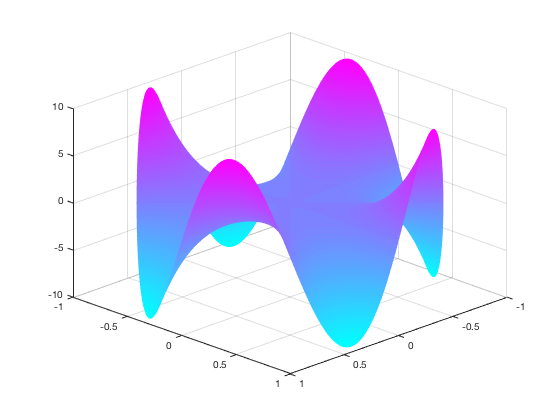
\includegraphics[width=5cm]{images/swing_function_plot.png}
  \caption{$u(x)$}%{Numerically solved solution}
  \label{fig:swingPlot}
\end{figure}


Equations can also be labeled
\begin{equation}
    \pi = \mathrm{e}^{i\cdot\phi}
    \label{eq:equation1}
\end{equation}


And later referenced. Even in subfigures.
\begin{figure}[!htb]
  \centering
  \begin{subfigure}[b]{0.3\textwidth}
    \centering
  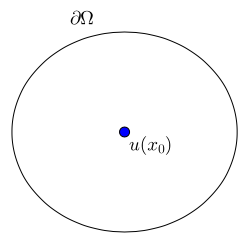
\includegraphics[width=\textwidth]{images/CircCenter}
  \caption{Equation \ref{eq:equation1}}\label{fig:circcenter}
\end{subfigure}
\hfill
  \begin{subfigure}[b]{0.3\textwidth}
    \centering
  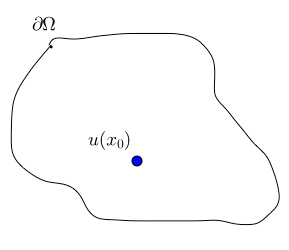
\includegraphics[width=\textwidth]{images/GeneralOffset}
  \label{fig:generaloffset}
  \caption{Equation \ref{eq:equation1}}
\end{subfigure}
\end{figure}
\section{Including code}

Code can be using the package
\href{https://www.sharelatex.com/learn/Code\_Highlighting\_with\_minted}{Minted}.

An exaple of which of can be found below (see Source Code \ref{lst:nice_listing})
\begin{listing}
    %the language syntax can be declared here.
    \begin{minted}{python}
    import numpy as np

    def incmatrix(genl1,genl2):
        m = len(genl1)
        n = len(genl2)
        M = None #to become the incidence matrix
        VT = np.zeros((n*m,1), int)  #dummy variable

        #compute the bitwise xor matrix
        M1 = bitxormatrix(genl1)
        M2 = np.triu(bitxormatrix(genl2),1)

        for i in range(m-1):
            for j in range(i+1, m):
                [r,c] = np.where(M2 == M1[i,j])
                for k in range(len(r)):
                    VT[(i)*n + r[k]] = 1;
                    VT[(i)*n + c[k]] = 1;
                    VT[(j)*n + r[k]] = 1;
                    VT[(j)*n + c[k]] = 1;

                    if M is None:
                        M = np.copy(VT)
                    else:
                        M = np.concatenate((M, VT), 1)

                    VT = np.zeros((n*m,1), int)

        return M
    \end{minted}

  \caption{My nice listing}
  \label{lst:nice_listing}
\end{listing}


%
%% ---------------------------------------------------------------------------
%%
%% Thesis content: What did you do?
%%
%%% ---------------------------------------------------------------------------
\part[Body: What was done for the thesis]{Body: What Was Done for the Thesis}
\label{part:body}

%% ---------------------------------------------------------------------------
%%
%% Results and Conclusion
%%
%% ---------------------------------------------------------------------------
\part[Results and Conclusion]{Results and Conclusion}
\label{part:resultsAndConclusion}


% ---------------------------------------------------------------------------
%
% Appendix
%
% ---------------------------------------------------------------------------
\part*{Appendix}
\phantomsection
\addcontentsline{toc}{part}{Appendix}

\appendix %---------------------------------------

% !TEX root = ../main.tex
\chapter{Detailed Descriptions}
%\section{Detailed Validation Results}
\label{chapter:DetailedDescriptions}\label{appendix}
%\inputminted{c++}{../../src/wos_native.cuh}
\newpage




 \clearemptydoublepage
 \printglossaries
 \bibliography{bibliography/literature}

\end{document}
